\documentclass{beamer}

% choose theme (warning, to use the UniBern theme you need to copy the files beamerthemeUniBern.sty and ublogo.pdf in the same directory)
\usetheme{UniBern}

% packages

\usepackage{graphicx}
\usepackage{hyperref} % allows clickable urls
\usepackage{tikz}
\usepackage{listings} % show code

\newcommand\blfootnote[1]{%
	\begingroup
	\renewcommand\thefootnote{}\footnote{#1}%
	\addtocounter{footnote}{-1}%
	\endgroup
}

% define title page
\title{Bayesian workflow for disease transmission modeling in Stan}
\subtitle{{\small Eustat -- XXXIII International Statistical Seminar} }
\author{Julien Riou, MD PhD}
\date{Institute of Social and Preventive Medicine, University of Bern, Switzerland}
\institute{institute}

% begin document
\begin{document}
	
\frame{\titlepage}

\frame{
	\frametitle{Preface}
	\begin{itemize}
		\item Objective: fit transmission models in Stan 
		\item Based on Grinsztajn et al., 2020 (\underline{\href{https://arxiv.org/abs/2006.02985}{link}})
		\item Prerequisites:
			\begin{itemize}
				\item general understanding of Bayesian inference
				\item basic programming with \texttt{R} and \texttt{Stan}
			\end{itemize}
		\item All material is available on \url{https://github.com/jriou/bayesian_workflow}
	\end{itemize}
}

\frame{
	\frametitle{Outline}
	\begin{itemize}
		\item Introduction
%		\item (Quick notice: Bayesian inference)
		\item (Quick notice: Bayesian inference with Stan)
		\item Simple SIR
		\item Using simulated data
		\item Scaling up ODE-based models
		\item Extensions 
	\end{itemize}
	
	\vspace{4em}
	\blfootnote{Ref: Grinsztajn et al.~(2020)}
}

\frame{
	\frametitle{Introduction}
	Models of disease transmission:
	\begin{itemize}
		\item Interpretability: mechanistic, phenomenological
		\pause
		\item Data-generating mechanisms: incubation, contagion, immunity...
		\pause
		\item Scale: agent-based, population-based
		\pause
		\item Framework: deterministic, stochastic
	\end{itemize}
	\pause
	
	\vspace{2em}
	Mechanistic + population-based + deterministic 
	
	\vspace{1em}\hspace{2em} $\rightarrow$ \alert{ODE-based compartmental model} (e.g., SIR)
}

\frame{
	\frametitle{Introduction}
	ODE-based compartmental model:
	\begin{itemize}
		\item Divide the population into homogeneous groups (compartments)
		\pause
		\item Define flows between compartments with differential equations
		\pause
		\item Define initial conditions
		\pause
		\item Solve for the time-dependent volume in each compartment
	\end{itemize}
	\vspace{1em}
	\pause
	
	\begin{figure}
		\centering
		\scalebox{.8}{
		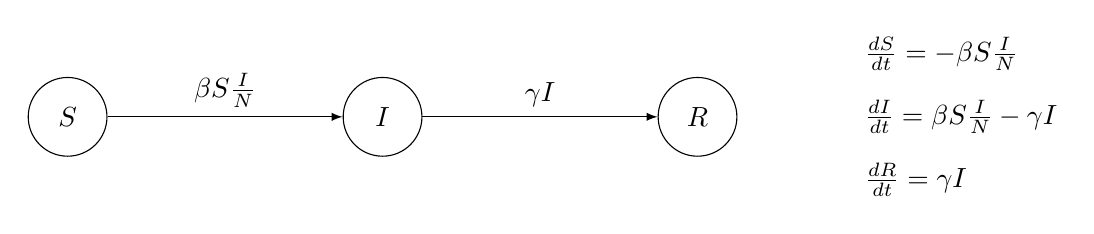
\begin{tikzpicture}
			\node[circle, draw, inner sep=0pt, minimum size=1cm] (S) at (0,0) {$S$};
			\node[circle, draw, inner sep=0pt, minimum size=1cm] (I) at (4,0) {$I$};
			\node[circle, draw, inner sep=0pt, minimum size=1cm] (R) at (8,0) {$R$};
			
			\draw[->,>=latex] (S) edge node[above] { $\beta S \frac{I}{N}$} (I);
			\draw[->,>=latex] (I) edge node[above] { $\gamma I$} (R);
			
			\node[anchor=west] at (10,.8) {$	\frac{dS}{dt} = - \beta S \frac{I}{N}$};
			\node[anchor=west] at (10,0) {$	\frac{dI}{dt} = \beta S \frac{I}{N} - \gamma I $};
			\node[anchor=west] at (10,-.8) {$\frac{dR}{dt} = \gamma I $};
		\end{tikzpicture}
	}
	\end{figure}
}


\frame{
	\frametitle{Introduction}
	
	Simulate in \texttt{R} with package \texttt{deSolve}:
	
	\begin{itemize}
		\item set compartments and differential equations
	\end{itemize}
	\begin{figure}
		\centering
		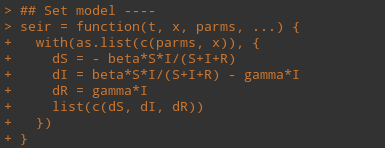
\includegraphics[width=0.55\linewidth]{simple_sir/simsir3.png}
	\end{figure}
	\pause
	\begin{itemize}
		\item set (fixed) values for $\beta$, $\rho$ and initial conditions
		
		 $\beta=0.8$; $\gamma=1/7$; $S(0)=100,000-50$; $I(0)=50$; $R(0)=0$
	\end{itemize}
	\begin{figure}
		\centering
		
\includegraphics[width=0.45\linewidth]{simple_sir/simsir1.png}
		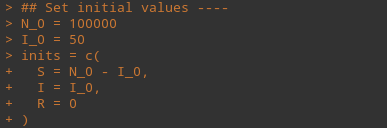
\includegraphics[width=0.45\linewidth]{simple_sir/simsir2.png}
	\end{figure}
}


\frame{
	\frametitle{Introduction}
	\begin{itemize}
		\item solve the ODE system numerically (Runge-Kutta 4th order)
	\end{itemize}
	\begin{figure}
		\centering
		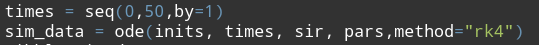
\includegraphics[width=0.7\linewidth]{simple_sir/simsir4.png}
	\end{figure}
}

\frame{
	\frametitle{Introduction}
	\begin{itemize}
		\item we obtain (deterministic) values for $S(t)$, $I(t)$ and $R(t)$
	\end{itemize}
	
	\begin{figure}
		\centering
		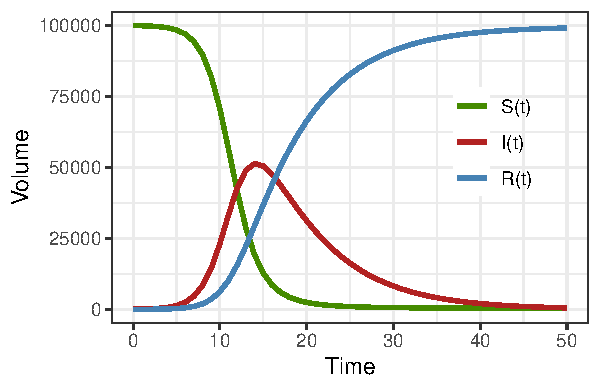
\includegraphics[width=0.7\linewidth]{simple_sir/example_sir1.pdf}
	\end{figure}

	\begin{itemize}
		\item these quantities have real-world interpretations (respectively susceptibility, prevalence, and cumulative attack rate)
	\end{itemize}
}

\frame{
	\frametitle{Introduction}
	\begin{itemize}
		\item the result is entirely determined by the chosen values for $\beta$, $\rho$ and the initial conditions
	\end{itemize}
	
	\begin{figure}
		\centering
		\only<1>{
			with $\beta = 1.1$ instead of $0.8$, we get \\
			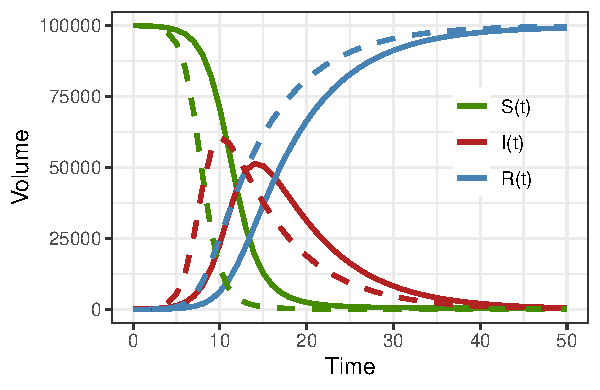
\includegraphics[width=0.7\linewidth]{simple_sir/example_sir2.pdf}
		}
		\only<2>{
			with $\beta = 0.6$ instead of $0.8$, we get \\
			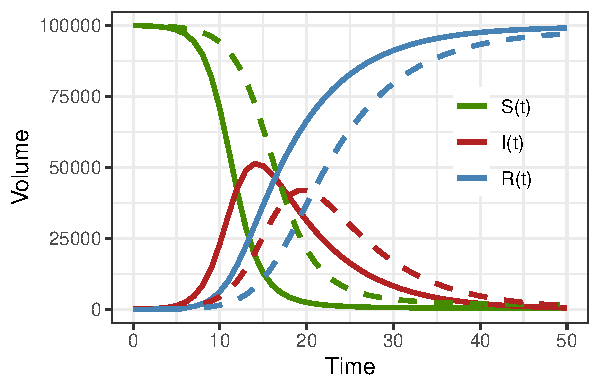
\includegraphics[width=0.7\linewidth]{simple_sir/example_sir3.pdf}
		}
		\only<3>{
		with $\gamma = 1/14$ instead of $1/7$, we get \\
		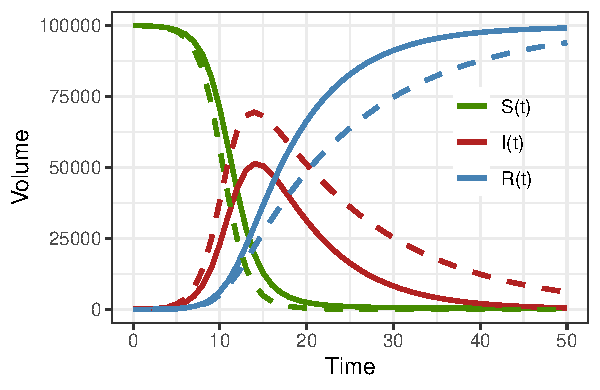
\includegraphics[width=0.7\linewidth]{simple_sir/example_sir4.pdf}
		}
		\only<4>{
		with $\gamma = 1/4$ instead of $1/7$, we get \\
		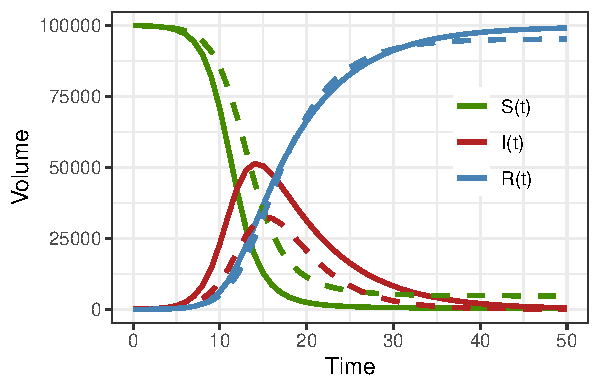
\includegraphics[width=0.7\linewidth]{simple_sir/example_sir5.pdf}
		}
		\only<5>{
		with $I(0) = 500$ instead of $50$, we get \\
		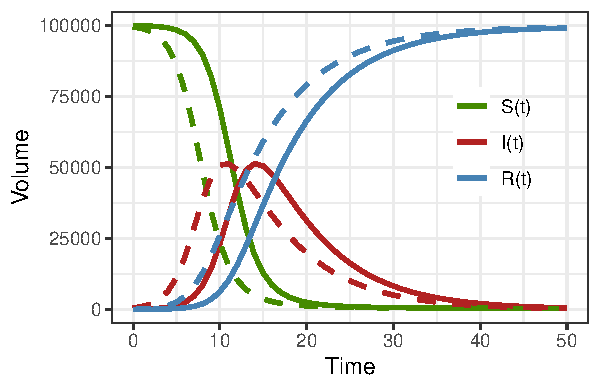
\includegraphics[width=0.7\linewidth]{simple_sir/example_sir6.pdf}
		}
		\only<6>{
		with $I(0) = 5$ instead of $50$, we get \\
		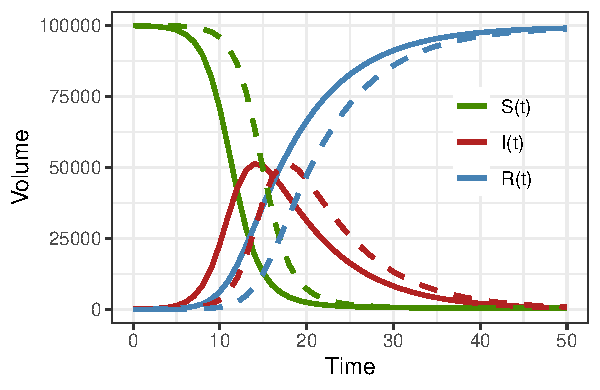
\includegraphics[width=0.7\linewidth]{simple_sir/example_sir7.pdf}
		}
		\only<7>{
		with $R(0) = 20,000$ instead of $0$, we get \\
		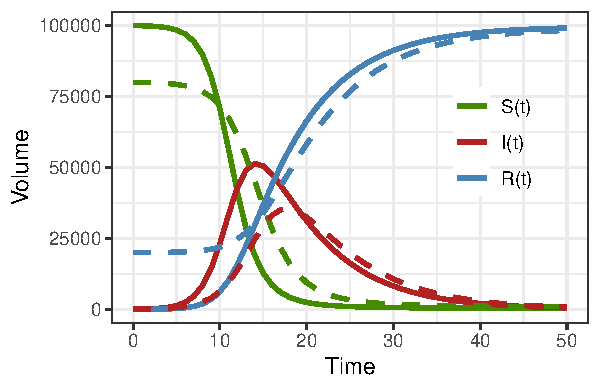
\includegraphics[width=0.7\linewidth]{simple_sir/example_sir8.pdf}
		}
	\end{figure}
}

\frame{
	\frametitle{Introduction}
	Compartmental models have many uses:
	\begin{itemize}
		\item formalize and quantify general concepts (herd immunity, vaccination threshold...)
		\item get mechanistic insight about an epidemic ($\mathcal{R}_0$, $\mathcal{R}_t$, impact of interventions...)
		\item produce forecasts (based on mechanisms)
	\end{itemize}
	
	\pause\vspace{2em}
	$\rightarrow$ based on \alert{numerical values for $\beta$, $\rho$ and the initial conditions}
}

\frame{
	\frametitle{Introduction}
	Enters \alert{Bayesian inference}:
	\begin{itemize}
		\item make the best use of information from data
		\item easily incorporate prior knowledge
		\item infer the value (posterior) of the parameters
		\item propagate uncertainty from data and priors
	\end{itemize}
	
	\pause\vspace{2em}
	$\rightarrow$ Markov Chain Monte Carlo methods and \alert{Stan}
}


\frame{
	\frametitle{(Bayesian inference with Stan)}
	General principle of Bayesian inference:
	\begin{itemize}
		\item specify a \alert{complete Bayesian model}
		\begin{itemize}
			\item[-] consider data $y = \{y_1,...,y_n\}$ and parameter $\theta$
			\item[-] specify an observation model $$\Pr(y|\theta) = \prod_n \text{normal}(y_n | \theta,1)$$
			\item[-] complete the model with a prior on the parameter $$\Pr(\theta) = \text{normal}(0,1)$$
		\end{itemize}
%		\item estimate the \alert{posterior distribution of $\theta$} 
%		$$ \Pr(\theta|y) = \frac{\Pr(y|\theta) \Pr(\theta)}{\Pr(y)}  $$
		\item estimate the \alert{joint probability density function} of the model
	\end{itemize}
}

\frame{
	\frametitle{(Bayesian inference with Stan)}
	The \alert{joint probability density function} of the model is given by
		$$
		\Pr(y, \theta)
		=
		\prod_{n = 1}^{N} \text{normal\_pdf} \, (y_{n} \mid \theta, 1)
		\cdot \text{normal\_pdf} \, (\theta \mid 0, 1)
		$$
	or on the log scale
	$$
	\log \Pr(y, \theta)
	=
	\sum_{n = 1}^{N} \text{normal\_lpdf} \, (y_{n} \mid \theta, 1)
	+ \text{normal\_lpdf} \, (\theta \mid 0, 1) 
	$$
}

\frame{
	\frametitle{(Bayesian inference with Stan)}
	Programming in Stan is structured in \alert{blocks}:
	\begin{itemize}
		\item the \texttt{data} block defines data variables
		\begin{figure}
			\centering
			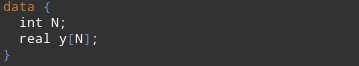
\includegraphics[width=0.6\linewidth]{example_linear/example_linear1.png}
		\end{figure}
		
		\item the \texttt{parameters} block defines parameters
		\begin{figure}
			\centering
			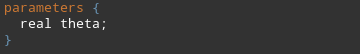
\includegraphics[width=0.6\linewidth]{example_linear/example_linear2.png}
		\end{figure}
		
		\item the \texttt{model} block defines the \alert{target log probability density function}
		\begin{figure}
			\centering
			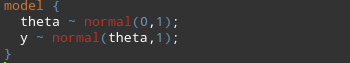
\includegraphics[width=0.6\linewidth]{example_linear/example_linear3.png}
		\end{figure}
	
	\end{itemize}
	
}

\frame{
	\frametitle{(Bayesian inference with Stan)}
	We then explore the target with \alert{Hamiltonian Monte Carlo}:
	\begin{itemize}
		\item load \texttt{rstan} package
		\begin{figure}
			\centering
			
\includegraphics[width=0.7\linewidth]{example_linear/run_stan1.png}
		\end{figure}
		
		\item simulate $N=50$ data points with $\theta=0.7$
		\begin{figure}
			\centering
			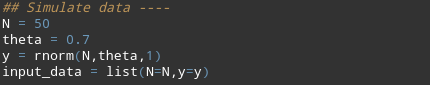
\includegraphics[width=0.7\linewidth]{example_linear/run_stan2.png}
		\end{figure}
		
		\item run sampling
		\begin{figure}
			\centering
			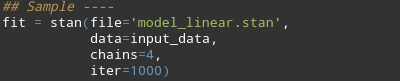
\includegraphics[width=0.7\linewidth]{example_linear/run_stan3.png}
		\end{figure}
	\end{itemize}
}

\frame{
	\frametitle{(Bayesian inference with Stan)}

	\begin{itemize}
		\item print results
		\begin{figure}
			\centering
			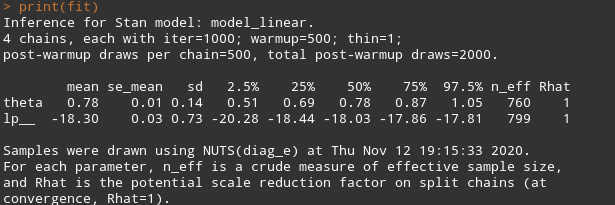
\includegraphics[width=.9\linewidth]{example_linear/run_stan4.png}
		\end{figure}
	\item diagnostics: $\hat{R}$, divergences, tree depth, energy
	\begin{figure}
		\centering
		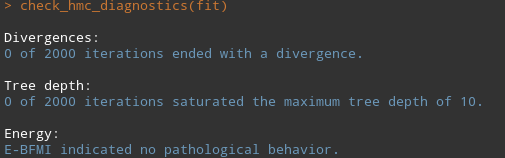
\includegraphics[width=.7\linewidth]{example_linear/run_stan5.png}
	\end{figure}
	\end{itemize}
}


\frame{
	\frametitle{Acknowledgements \& ressources}
	\begin{itemize}
		\item Michael Betancourt's \textit{Introduction to Stan} \url{https://betanalpha.github.io/assets/case_studies/stan_intro.html}
		\item Daniel Lee's \textit{ODEs in Stan} \\ \url{https://youtu.be/hJ34_xJhYeY}
		\item Richard McElreath's \textit{Statistical rethinking} \url{https://youtu.be/4WVelCswXo4}
	
	\end{itemize}
}

\end{document}
